\documentclass[../main.tex]{subfiles}


\begin{document}
\raggedright
Data will eventually need to be stored in a database and to do a schema for a database must exist. Figure \ref{fig:dbschema} shows the schema created to store and retrieve data without bring up errors and making sure that the tables are interlinked. A single form can have multiple modules and files, similarly a single user can have multiple forms(One to Many). However, a single user can only have a one to one relationship with the users public data and profile. 

\begin{figure}[H]
        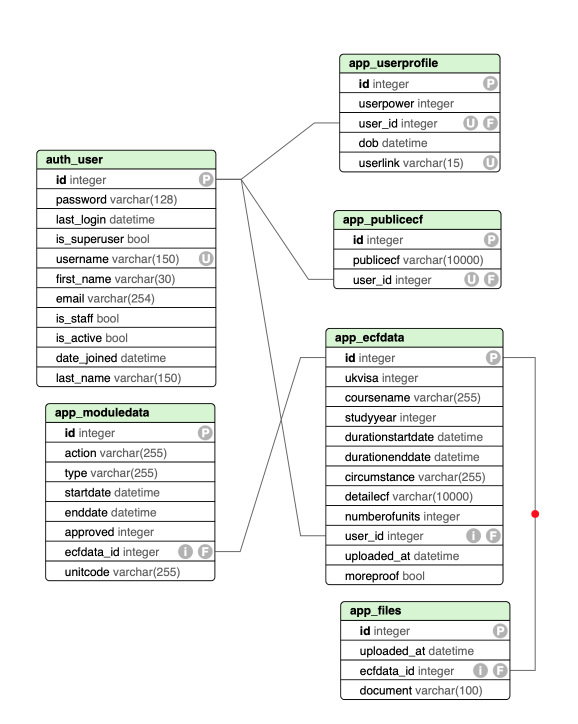
\includegraphics[scale=1.2]
        {images/db.png}
        \caption{\label{fig:dbschema} Database Schema}
      \end{figure}
  
  
\end{document}
